%%%%%%%%%%%%%%%%%%%%%%%%%%%%%%%%%%%%%%%%%%%%%%%%%%%%%%%%%%%%%%%%%%%%%%%%%%%%%%%%
%2345678901234567890123456789012345678901234567890123456789012345678901234567890
%        1         2         3         4         5         6         7         8

\documentclass[letterpaper, 10 pt, conference]{ieeeconf}  % Comment this line out
                                                          % if you need a4paper
%\documentclass[a4paper, 10pt, conference]{ieeeconf}      % Use this line for a4
                                                          % paper

\IEEEoverridecommandlockouts                              % This command is only
                                                          % needed if you want to
                                                          % use the \thanks command
\overrideIEEEmargins
% See the \addtolength command later in the file to balance the column lengths
% on the last page of the document

\usepackage[utf8]{inputenc}
\usepackage[T1]{fontenc}
\usepackage{graphicx}
\usepackage{float}
\usepackage{comment}

% The following packages can be found on http:\\www.ctan.org
%\usepackage{graphics} % for pdf, bitmapped graphics files
%\usepackage{epsfig} % for postscript graphics files
%\usepackage{mathptmx} % assumes new font selection scheme installed
%\usepackage{mathptmx} % assumes new font selection scheme installed
%\usepackage{amsmath} % assumes amsmath package installed
%\usepackage{amssymb}  % assumes amsmath package installed

\title{\LARGE \bf
Aplicação de GPUs no contexto da computação em nuvem e inteligência artificial}

%\author{ \parbox{3 in}{\centering Huibert Kwakernaak*
%         \thanks{*Use the $\backslash$thanks command to put information here}\\
%         Faculty of Electrical Engineering, Mathematics and Computer Science\\
%         University of Twente\\
%         7500 AE Enschede, The Netherlands\\
%         {\tt\small h.kwakernaak@autsubmit.com}}
%         \hspace*{ 0.5 in}
%         \parbox{3 in}{ \centering Pradeep Misra**
%         \thanks{**The footnote marks may be inserted manually}\\
%        Department of Electrical Engineering \\
%         Wright State University\\
%         Dayton, OH 45435, USA\\
%         {\tt\small pmisra@cs.wright.edu}}
%}

\author{Levy G. da S. Galvão$^{1}$ e Thiago M. Souto$^{2}$% <-this % stops a space
\thanks{*This work was not supported by any organization}% <-this % stops a space
\thanks{$^{1}$ Graduando em Engenharia Elétrica, Universidade Federal do Rio Grande do Norte, Brasil.}%
\thanks{$^{2}$ Graduando em Engenharia Elétrica, Universidade Federal do Rio Grande do Norte, Brasil.}%
}


\begin{document}



\maketitle
\thispagestyle{empty}
\pagestyle{empty}


%%%%%%%%%%%%%%%%%%%%%%%%%%%%%%%%%%%%%%%%%%%%%%%%%%%%%%%%%%%%%%%%%%%%%%%%%%%%%%%%
\begin{abstract}

As unidade de processamento gráfico (GPUs) evoluíram a partir da necessidade de processamento gráfico tridimensional, atualmente possuindo aplicações de propósito geral em várias áreas: bioinformática, inteligência artificial (AI), jogos, \textit{data centers}, etc. Assim surge a necessidade de avaliar como a computação em nuvem e como as GPUs desempenham um papel fundamental para suprir a demandas de áreas que estão exigindo cada vez mais processamento. Este trabalho se propõe a apresentar algumas características que tornam as GPUs ideais para aplicação em \textit{data centers} e pretende contextualizar algumas aplicações de computação em nuvem e AI que impactam a forma como a tecnologia está se desenvolvendo.

\end{abstract}


%%%%%%%%%%%%%%%%%%%%%%%%%%%%%%%%%%%%%%%%%%%%%%%%%%%%%%%%%%%%%%%%%%%%%%%%%%%%%%%%
\section{INTRODUÇÃO}

A diversidade de aplicações que são executadas em \textit{data centers} modernos levou a uma explosão no uso de unidades de processamento gráfico (GPUs) na aceleração da computação em nuvem. Essas aplicações incluem as mais diversas cargas de trabalho, entre elas: o treinamento e inferência do aprendizado profundo de inteligências artificiais (AI); análise de dados; processamento gráfico; computação cientifica; análise genética; análise de ponta em vídeos; redes 5G; jogos em nuvem, entre outras. 

Essas aplicações demandam um intenso processamento que é fornecido por GPUs com arquiteturas específicas para lidar com tais tarefas.

Enquanto que se diferenciam as GPUs entre integradas e dedicadas, sendo estas \textit{chips} totalmente separados da CPU, enquanto que aquelas estão presentes no mesmo chip que a CPU. Também existem outras diferenciações para aquelas que são dedicadas. 

As GPUs dedicadas podem ser divididas entre aquelas voltadas para estações de trabalho e PCs, que geralmente possuem um preço mais acessível ao usuário; enquanto que também existem GPUs voltadas para \textit{data centers} e que atuam, especificamente, em sistemas de \textit{cloud computing} que possuem uma maior robustez e preço. 

Isso não significa dizer que apenas GPUs de arquitetura voltada para \textit{data centers} são utilizadas para treinamento de inteligências artificiais. Significa dizer que elas são otimizadas para esse tipo de aplicação, seja possuindo mais blocos voltados para uma alta taxa de processamento algébrico ou abdicando de blocos que são específicos para processamento e apresentação gráfica.

Dessa forma, este trabalho irá avaliar algumas características básicas de arquiteturas de GPUs voltadas para computação em nuvem. Também serão avaliados os desafios e soluções exigidas pelas aplicações modernas em computação em nuvem.

\section{CARACTERÍSTICAS DAS ARQUITETURAS DE GPU PARA \textit{DATA CENTERS}}

Uma grande adição à cena das GPUs para a computação em nuvem foi a introdução dos poderosos \textit{Tensor Cores} (TC) da NVIDIA, em 2017. Os TCs são ALUs especializadas em operações matriciais e lidam com dados FP16, INT8 ou INT4, de forma que em um ciclo de clock ocorram até 64 operações de multiplicar-depois-somar. Isso permite que operações matriciais sejam feitas enquanto os CUDA cores (ou RT cores, caso existam) realizam outras operações. 

A GPU Tesla V100 da microarquitetura Volta foi a primeira a possuir esses blocos. Eles promovem uma tremenda aceleração na computação de matrizes, funcionando como o coração de operações de treinamento e inferência no aprendizado profundo de redes neurais. Em 2018, as GPUs Tesla T4 da NVIDIA, utilizando os TCs da microarquitetura Turing trouxeram uma significante aceleração para \textit{data centers}, se preocupando com eficiência energética. Os TCs da arquitetura Turing também permitiram que recursos de AI fossem implementados em PCs de jogos (família GeForce) e estações de trabalho (família Quadro), uma vez que esses dispositivos são o foco dessa microarquitetura.

No \textit{whitepaper} da microarquitetura Ampere da NVIDIA é apresentado um quadro comparativo entre \textit{chips} dessa futura geração, da microarquitetura Volta para \textit{data centers} e da microarquitetura Pascal para uso pessoal. Alguns dados desse quadro estão presentes na tabela \ref{table:1}.

\begin{table}[h]
\centering
\caption{\textit{Comparativo entre chips Pascal, Volta e Ampere da NVIDIA.}}\label{table:1}
\begin{tabular}{|l|l|l|l|} \hline
Características das GPUs & Tesla P100 & Tesla V100 & A100 \\ \hline
Microarquitetura & Pascal & Volta & Ampere \\ \hline
SMs & 56 & 80 & 108 \\ \hline
Cores FP32/GPU & 3584 & 5120 & 6912 \\ \hline
Cores FP64/GPU & 1792 & 2560 & 3456 \\ \hline
Cores INT32/GPU & NA & 5120 & 6912 \\ \hline
Tensor Core/GPU & NA & 640 & 432 \\ \hline
Tensor Core/SM & NA & 8 & 16 \\ \hline
Tamanho da memória & 16 GB & 32 GB / 16 GB & 40 GB \\\hline
Larg. Bnd. da memória & 720 GB/s & 900 GB/s & 1555 GB/s \\ \hline
Tamanho da cache L2 & 4096 KB & 6144 KB & 40960 KB \\ \hline
\end{tabular}
\end{table}

A tabela \ref{table:1} deixa bem clara a evolução em termos de blocos computacionais e características de memória das gerações da NVIDIA. Vale destacar o aumento das ALUs e SMs, bem como o surgimento dos Tensor Cores na arquiteturas para \textit{data centers}. 

É inevitável notar que o número de TCs diminuiu da primeira geração no chip V100 para a terceira geração no chip A100. Isso se deve, pois a terceira geração de TCs (Ampere) possui o dobro da potência de computação em comparação com as gerações anteriores (primeira, na Volta e segunda, na Turing), pois acelera operações com todos os tipos de dados e explora a esparsidade estruturada de baixa granularidade em redes de \textit{deep learning}, entre outras características.

Em termos de AMD, foi revelada uma nova arquitetura AMD a ser lançada ainda no ano de 2020, a Compute DNA (CDNA). Esta arquitetura é um ramificação da arquitetura Radeon DNA (RDNA) destinada a jogos e é projetada especialmente para acelerar o desempenho da carga de trabalho dos \textit{data centers}. A eficiência em quesitos de GPUs para \textit{data centers} se deve, pois a arquitetura não necessita de tantos recursos que uma placa gráfica tem para consumidores normais, como a renderização e apresentação de \textit{pixels} e \textit{ray tracing}. (RYAN, 2020)

A arquitetura CDNA inclui a segunda geração do AMD \textit{Infinity Architecture} para melhorar a conectividade entre GPUs e é otimizada para alto desempenho em aplicações de aprendizado de máquina. A programação é de que até 2022 seja lançada a arquitetura CDNA 2 que dará suporte à terceira geração da AMD \textit{Infinity Architecture} para habilitar a capacidade de computação da ordem de exa FLOPS ($10^{18}$ FLOPS) para a próxima geração de supercomputadores (as tecnologias atuais estão na escala de tera FLOPS). (YOUNGBAUER \& GRAVES, 2020)

\section{APLICAÇÕES DE COMPUTAÇÃO EM NUVEM E INTELIGÊNCIA ARTIFICIAL}

Nesta seção será apresentado um recorte de três aplicações que envolvem computação em nuvem e$/$ou inteligência artificial e que exigem uso intensivo de GPUs, além de estimular sua evolução.

\subsection{Jogos em nuvem: Google Stadia}

O Google Stadia é um serviço de jogos em nuvem desenvolvido e mantido pela Google. A proposta do serviço é oferecer uma plataforma de jogos na qual todo o processamento relacionado aos jogos dos usuários seja realizado em \textit{data centers} da Google. De acordo com a Google, o serviço oferece suporte à resolução de 4K a 60 FPS e com som \textit{surround} e HDR. No futuro a Google pretende dar suporte à resolução de 8K e com 120 FPS. (CONNATSER, 2019)

As GPUs utilizadas para esse serviço surgiram da parceria entre Google e AMD para desenvolver uma GPU especializada para seus \textit{data centers}. De forma que a primeira geração da plataforma da Stadia utilizava GPUs Vega 56 de 14nm com arquitetura GCN 1.5 com 56 \textit{Compute Units} (CU), largura de banda de memória de 484 GB/s e 10.7 TFLOPS.

Pela quantidade de CUs, essa GPU aparenta ser uma versão customizável voltada para \textit{data centers} do chip Vega 56, porém a alta largura de banda de memória, no que é esperado ser de 8 GB de HBM2 VRAM (\textit{High Bandwidth Memory}), junto com 8 GB de DRAM, tenta acompanhar os moldes do chip Vega 64. 

Algumas comparações podem ser feitas com placas de outras microarquiteturas da AMD e até com algumas da NVIDIA. Por exemplo, a Radeon RX 5700 XT da AMD que implementa a arquitetura RDNA e microarquitetura Navi possui 40 CUs e uma largura de banda de memória de 448 GB/s e é voltada para PCs. A GeForce RTX 2070 da NVIDIA que implementa a microarquitetura Turing com o chip TU106 possui, também, largura de banda de 448 GB/s e é voltada para PCs. Enquanto que para arquiteturas para \textit{data centers} da NVIDIA, a Tesla V100 (Volta) e o A100 (Turing) possuem largura de banda de memória de, respectivamente, 900 GB/s e 1555 GB/s. Isso mostra que a Google não se importa de utilizar uma versão mais antiga em troca de estabilidade para a aplicação em \textit{data center}.

Outro fato importante é que, como a aplicação vai ser executada em um \textit{data center}, será permitido alocar múltiplas GPUs para uma instância de jogo, não significando apenas duas, mas quantas forem necessárias para manter o desempenho ideal ao usuário. 

Porém, uma das limitações é que o usuário deve dispor de uma rápida e estável conexão com a internet para manter contato frequente com os servidores da Google.

\subsection{Redução de custos para \textit{deep learning}}

Apesar de placas de processamento gráfico se tornarem cada vez mais necessárias na computação, isso não significa dizer que elas sejam uma \textit{commoditie} barata, na verdade, está longe disso. Considerando a AMD RX 5700-XT lançada em Q3 2019 que possui um preço razoável de R\$ 1,399, porém ainda alto, existem placas da NVIDIA, como a RTX 2080-Ti que chegam a custar cerca de R\$5,000 e sua antecessora GTX 1080-Ti de cerca de R\$3,000 que representam uma cifra ainda maior.

Para aqueles que não são artistas que renderizam gráficos constantemente ou \textit{gamers} amadores ou profissionais que necessitam de altas taxas de \textit{frames}, entre outros, adquirir uma GPU não vale a pena. O mercado reconhece esse público e possui soluções de aluguel de processamento por GPU para usuários casuais que necessitem de um poder de processamento maior em apenas alguns momentos.

HALE (2018) realizou alguns testes com provedores de GPU em nuvem que propõem soluções para um grande subconjunto de profissionais no ambiente de aprendizado profundo e avaliou-os com o objetivo de determinar uma comparação de preço em função da rapidez do serviço. Estes são:

\begin{itemize}
    \item Google Colab (gratuito, possui GPU e TPU);
    \item Google Cloud (mais poderoso que o Colab, com interface amigável, TPUs e um preço difícil de estimar);
    \item AWS (escalável, seguro, confiável e não é tão fácil de configurar; a oferta de GPU de nível básico é a p2.xlarge, que instancia um servidor virtual atrvés do Amazon Elastic Compute Cloud com placas NVIDIA Tesla K80 com 4 CPUs e 61 RAM.);
    \item Paperspace (possui TPUv2s disponíveis e são caras neste caso se comparadas com a Google Cloud);
    \item vast.ai (propõe o uso de GPUs de terceiros que listam suas máquinas na plataforma e costuma possuir preços bons; teoricamente esses terceiros podem acessar os dados do usuário, mas não facilmente.);
\end{itemize}

As unidades de processamento tensorial (TPU) são responsáveis pelo aceleramento de aplicações em AI e foram desenvolvidas pela Google e usam o próprio aplicativo TensorFlow da Google. A discussão desse ASIC e comparação com CPU e GPU merece espaço em outros trabalhos devido sua substancial evolução.

Os provedores escolhidos representam apenas um recorte com o objetivo de comparação para o autor, porém existem vários outros no mercado.

\begin{comment}
O maior benefício do Google Colab é sua gratuidade.Ele também integra-se com o GitHub e o Google Drive. Ele possui GPU e unidade de processamento tensorial (TPU, responsável pelo aceleramento de aplicações em AI). O Google Cloud é um motor computacional mais poderoso que o Colab, com interface amigável, TPUs e um preço difícil de estimar. O AWS não é tão fácil de configurar, diferente do Cloud. A oferta de GPU de nível básico é a p2.xlarge, que instancia um servidor virtual através do Amazon Elastic Compute Cloud (EC2) com placas NVIDIA Tesla K80 com 4 CPUs, 61 GiB de memória principal e 12 GiB de memória gráfica. O provedor é escalável, seguro e confiável. Similarmente ao Google, a Paperspace também possui TPUv2s disponíveis e são caras neste caso se comparadas com a Google Cloud. O vast.ai é uma opção diferente das outras, pois propõe o uso de GPUs de terceiros que listam suas máquinas na plataforma e costuma possuir preços bons. Teoricamente esses terceiros podem acessar os dados do usuário, mas não facilmente.
\end{comment}

O autor propôs um experimento para um modelo de aprendizado profundo no classificador de imagem de cachorro e gato usando a FastAI v1.0 em um Jupyter Notebook. Dessa forma ele construiu o gráfico da figura \ref{medium:1} comparando os diversos provedores supracitados.

\begin{figure}[H]
\begin{center}
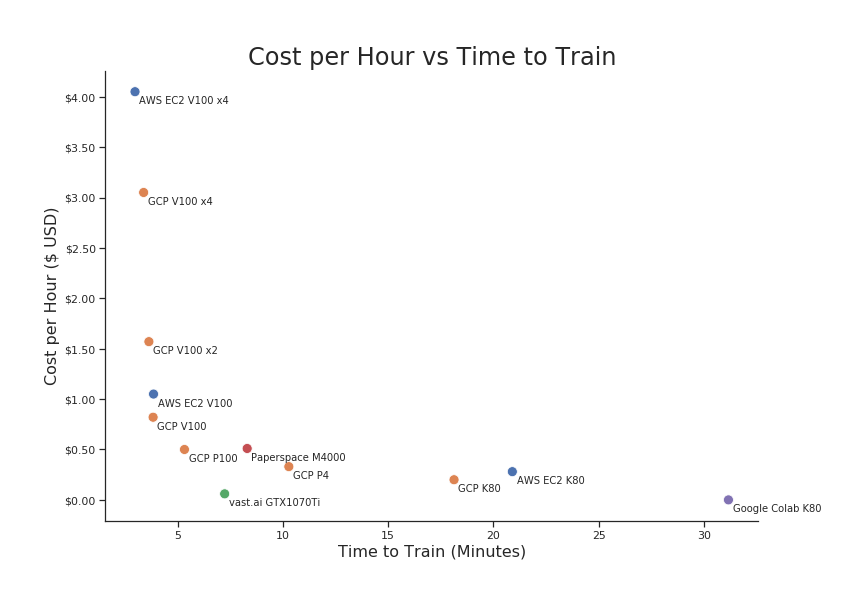
\includegraphics[width=8.5cm]{medium1.png}
\caption{Custo por hora vs. tempo de treinamento para diferentes provedores e diferentes GPUs da NVIDIA. Fonte: HALE (2018).}
\label{medium:1} 
\end{center}
\end{figure}

Na figura, o local desejável é o canto inferior esquerdo, que representa aqueles provedores e placas que possuíram um tempo pequeno de treinamento a um baixo custo. Nessa posição, além do Google Cloud, vale destacar o baixo custo e rapidez do vast.ai com uma placa GTX 1070Ti (NVIDIA Pascal), decorrente da plataforma que facilita a relação entre o usuário com terceiros dispostos a compartilhar suas placas de vídeo. (HALE, 2018)

Porém, também é importante avaliar os dois extremos: caro e rápido contra barato e lento. O AWS com o V100 (NVIDIA Volta) se mostrou bastante caro porém com um tempo desejável para aqueles que visam velocidade, denotando um provedor de uso mais profissional, enquanto o Google Colab com o Tesla K80 (NVIDIA Kepler, uma microarquitetura um pouco mais antiga, lançada em 2012), por ser gratuito possui um tempo maior de treinamento (30 min), ideal para aqueles que querem treinar suas primeiras redes neurais. O Google Cloud e o AWS com a placa K80 possuem um tempo de treinamento de 10 min menor que o Colab (média de 20 min no total), porém, pelo preço ainda compensa usar o Colab para iniciantes ou outras placas mais modernas em outros provedores para um desempenho mais profissional. (HALE, 2018) 

\subsection{Tecnologia de carros autônomos}

Veículos autônomos se propõem como uma solução para estradas seguras e mais eficientes com carros capazes de tomar decisões próprias. Porém, aliado a esses benefícios revolucionários, está associada a necessidade de um poder computacional massivo e a experiência em produção de software em larga escala.

A NVIDIA oferece soluções nessa área, abrangendo o desenvolvimento de veículos autônomos da nuvem para o carro, ajudando os fabricantes a coletar dados, treinar redes neurais profundas e testar, validar, e operar carros autônomos com as plataformas da NVIDIA DRIVE. 

Além da interface de \textit{software} voltada para aplicações customizadas em veículos autônomos, a NVIDIA DRIVE AGX se propõe como uma plataforma de computação em inteligência artificial. Aqui será explicado apenas um pouco das configurações do \textit{hardware}.

Um dos sistemas é o NVIDIA DRIVE AGX Xavier, capaz de entregar 30 trilhões de operações por segundo (TOPS). No seu núcleo há o Xavier SoC, que incorpora seis diferentes tipos de processadores para a execução de redundâncias e vários algoritmos para AI, processamento de sensores, mapeamento e direção. A NVIDIA diz que esse sistema é desenvolvido para nível 2+ para sistemas de assistência avançada em direção e nível 3 para direção automatizada. Outro sistema é o NVIDIA DRIVE AGX Pegasus. Este sistema aproveita o poder de dois SoC Xavier e duas GPUs NVIDIA Turing (microarquitetura mais nova) e é construída para nível 4 de alta automação em direção e nível 5 de direção autônoma e robo-taxis. Este sistema oferece 320 TOPS para operação sem motorista. Existe mais uma plataforma que é a NVIDIA DRIVE Hyperion que associa um Pegasus com sensores para testes e avaliações de software. (NVIDIA, 2019)

Em 2018, o CEO da Tesla, Elon Musk, anunciou o fim da parceria com a NVIDIA, abandonando a plataforma para veículos autônomos proferindo que sua empresa irá utilizar o próprio computador de inteligência artificial. Ele assumiu que os \textit{chips} são 10 vezes mais rápidos que os \textit{chips} da NVIDIA, argumentando que o uso de GPUs não é tão rápido e econômico quanto um \textit{chip} customizado (ASIC). Porém na época a plataforma da NVIDIA era a NVIDIA DRIVE PX 2 AI, com uma GPU da microarquitetura Pascal e dois processadores Parkers (CPUs) já ultrapassados pela atual. (SU, 2018)

A Google também desenvolvia sua própria tecnologia de veículos autônomos. A empresa é a Wyamo, parte da Alphabet. A Wyamo usa os \textit{data centers} da Google para treinar suas redes neurais. O\textit{ hardware} utilizado são os famosos TPUs da Google. Uma investida da Google para construir seu próprio \textit{hardware} e otimizá-lo para seu próprio software, assim não dependendo das GPUs da NVIDIA. (HAWKINS, 2018)

Apesar da área ter partido do campo da "possibilidade" para a "realidade" nos últimos anos, ainda existe muito a avançar, inclusive no que diz respeito à segurança dos usuários e pedestres, representando um dos maiores desafios da tecnologia. 

\section{CONCLUSÕES}

O mercado de GPUs possuem uma gama de variedades. Neste trabalho foi levado em conta apenas um recorte de aplicações que se apresentam de forma inovadora e ditam o passo de como a tecnologia de processamento gráfico deve ser no futuro.

Recursos adicionais em GPUs devem ser criticamente avaliados, pois como no caso do Ray Tracing da NVIDIA, alguns recursos podem não se adequar à aplicação, não significando que a tecnologia mais atual seja a ideal.

Soluções baratas podem custar caro por não atender a demanda da aplicação. Da mesma forma que uma solução cara pode comprometer o \textit{market share} do produto por ser inacessível ao usuário.

Finalmente, o profissional da área deve se manter atualizado com as novas arquiteturas de GPUs para poder compreender a mudança no contexto de sua aplicação. Porém é essencial conhecer as gerações anteriores para uma tomada de decisões mais ampla.



\addtolength{\textheight}{-12cm}   % This command serves to balance the column lengths
                                  % on the last page of the document manually. It shortens
                                  % the textheight of the last page by a suitable amount.
                                  % This command does not take effect until the next page
                                  % so it should come on the page before the last. Make
                                  % sure that you do not shorten the textheight too much.

%%%%%%%%%%%%%%%%%%%%%%%%%%%%%%%%%%%%%%%%%%%%%%%%%%%%%%%%%%%%%%%%%%%%%%%%%%%%%%%%



%%%%%%%%%%%%%%%%%%%%%%%%%%%%%%%%%%%%%%%%%%%%%%%%%%%%%%%%%%%%%%%%%%%%%%%%%%%%%%%%



%%%%%%%%%%%%%%%%%%%%%%%%%%%%%%%%%%%%%%%%%%%%%%%%%%%%%%%%%%%%%%%%%%%%%%%%%%%%%%%%
\begin{comment}


\section*{APPENDIX}

Appendixes should appear before the acknowledgment.

\section*{ACKNOWLEDGMENT}

The preferred spelling of the word ``acknowledgment'' in America is without an ``e'' after the ``g''. Avoid the stilted expression, ``One of us (R. B. G.) thanks . . .''  Instead, try ``R. B. G. thanks''. Put sponsor acknowledgments in the unnumbered footnote on the first page.



%%%%%%%%%%%%%%%%%%%%%%%%%%%%%%%%%%%%%%%%%%%%%%%%%%%%%%%%%%%%%%%%%%%%%%%%%%%%%%%%

References are important to the reader; therefore, each citation must be complete and correct. If at all possible, references should be commonly available publications.

\end{comment}

\begin{thebibliography}{99}


\bibitem{c} NVIDIA. NVIDIA Tesla V100 GPU architecture: The world's most advanced data center GPU. WP-08608-001v1.1. 2017
\bibitem{c} NVIDIA. NVIDIA Turing GPU architecture: Graphics reinvented. WP-09183-001v01. 2018
\bibitem{c} NVIDIA. NVIDIA A100 Tensor Core GPU Architecture: Unprecedented acceleration at every scale. V1.0. 2019
\bibitem{c} Youngbauer, Sarah e Graves, Laura. "AMD Details Strategy to Deliver Best-in-Class Growth and Strong Shareholder Returns at 2020 Financial Analyst Day." AMD, 3 May. 2020, https://www.amd.com/en/press-releases/2020-03-05-amd-details-strategy-to-deliver-best-class-growth-and-strong-shareholder
\bibitem{c} Connatser, Matthew. "Google Stadia to use First-Gen AMD Vega GPU Architecture: Khronos." tom's Hardware, 18 May. 2019, https://www.tomshardware.com/news/google-stadia-amd-vega-gpu,39375.html
\bibitem{c} James, Dave. "Google’s revolutionary Stadia tech is built on custom AMD GPUs" PCGames, 21 Mar. 2019, https://www.pcgamesn.com/amd/google-stadia-specs-custom-amd-gpu-x86-cpu
\bibitem{c} Maring, Joe e Tolbert, Samuel. "Stadia: What you need to know about Google's game streaming service." Android Central, 29 Jan. 2020, https://www.androidcentral.com/stadia
\bibitem{c} Smith, Ryan. "AMD Unveils CDNA GPU Architecture: A Dedicated GPU Architecture for Data Centers." Anand Tech, 5 Mar. 2020, https://www.anandtech.com/show/15593/amd-unveils-cdna-gpu-architecture-a-dedicated-gpu-architecture-for-data-centers
\bibitem{c} Condon, Stephanie. "AMD unveils new GPU architecture for data center compute workloads." ZD Net, 6 Mar. 2020, https://www.zdnet.com/article/amd-unveils-new-gpu-architecture-for-data-center-compute-workloads/
\bibitem{c} Warren, Tom e Vincent, James. "Nvidia’s first Ampere GPU is designed for data centers and AI, not your PC." The Verge, 14 May. 2020, https://www.theverge.com/2020/5/14/21258419/nvidia-ampere-gpu-ai-data-centers-specs-a100-dgx-supercomputer
\bibitem{c} Hale, Jeff. "Best Deals in Deep Learning Cloud Providers." Towards data science, 29 Oct. 2018, https://towardsdatascience.com/maximize-your-gpu-dollars-a9133f4e546a
\bibitem{c}  Su, Jeb. "Why Tesla Dropped Nvidia's AI Platform For Self-Driving Cars And Built Its Own." FORBES, 15 Aug. 2018, https://www.forbes.com/sites/jeanbaptiste/2018/08/15/why-tesla-dropped-nvidias-ai-platform-for-self-driving-cars-and-built-its-own/#6a335a296722
\bibitem{c} NVIDIA. "The Journey to Zero Accidents: NVIDIA DRIVE". May. 2019
\bibitem{c} Karkaria, Urvaksh. "New heart of the car: The GPU." Automotive News, 30 Jul. 2018, https://www.autonews.com/article/20180730/OEM10/180739942/new-heart-of-the-car-the-gpu
\bibitem{c} Hawkins, Andrew J. "Inside Waymo's straetgy to grow the best brains for self-driving cars." The Verge, 9 May. 2018, https://www.theverge.com/2018/5/9/17307156/google-waymo-driverless-cars-deep-learning-neural-net-interview
\end{thebibliography}




\end{document}
